\documentclass{X:/Documents/Coding/Latex/myreport}
\title{Brief Analysis of Norovirus Data}
\usepackage[style=numeric]{biblatex}
\addbibresource{sources.bib}

\begin{document}

\maketitle
Advise the government on effectiveness of interventions, and which should be implemented (if any). 


\begin{figure}[tb]
	\centering
	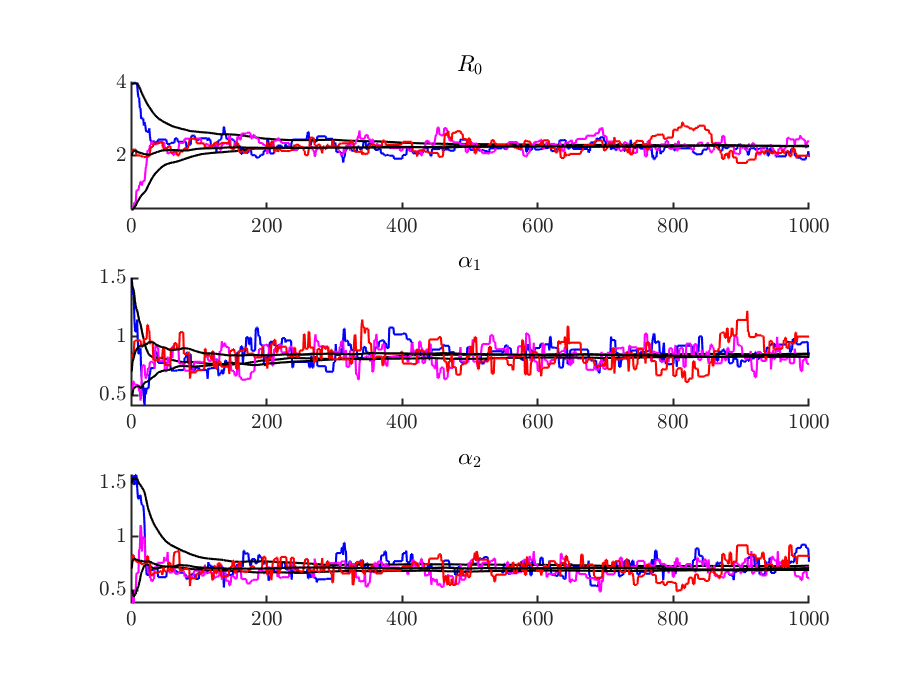
\includegraphics[width=\linewidth]{MHplot1.eps}
	\caption{Caption here}
	\label{fig:fullrun}
\end{figure}

\begin{figure}[tb]
	\centering
	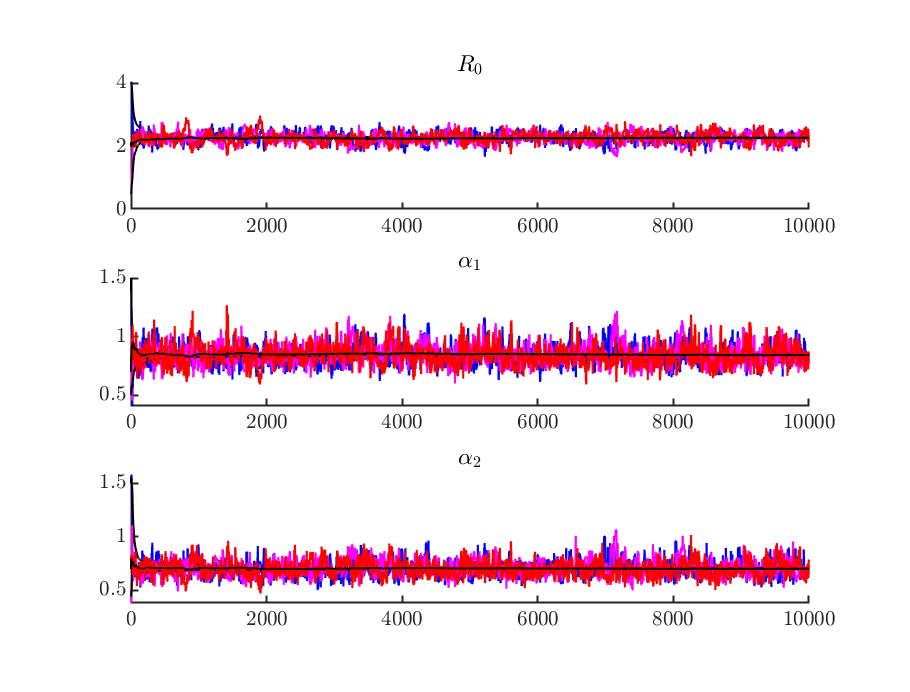
\includegraphics[width=\linewidth]{MHplot0.eps}
	\caption{Caption here}
	\label{fig:burnin}
\end{figure}





\clearpage
\appendix

\printbibliography
\section{Code}
\subsection{Main Script (R0Predict.m)}
\lstinputlisting{R0Predict.m}

\subsection{MetropolisHastingsPassLikelihood.m}
\lstinputlisting{MetropolisHastingsPassLikelihood.m}
\subsection{LogLikelihood.m}
\lstinputlisting{LogLikelihood.m}
\subsection{ProposalConstraints.m}
\lstinputlisting{ProposalConstraints.m}



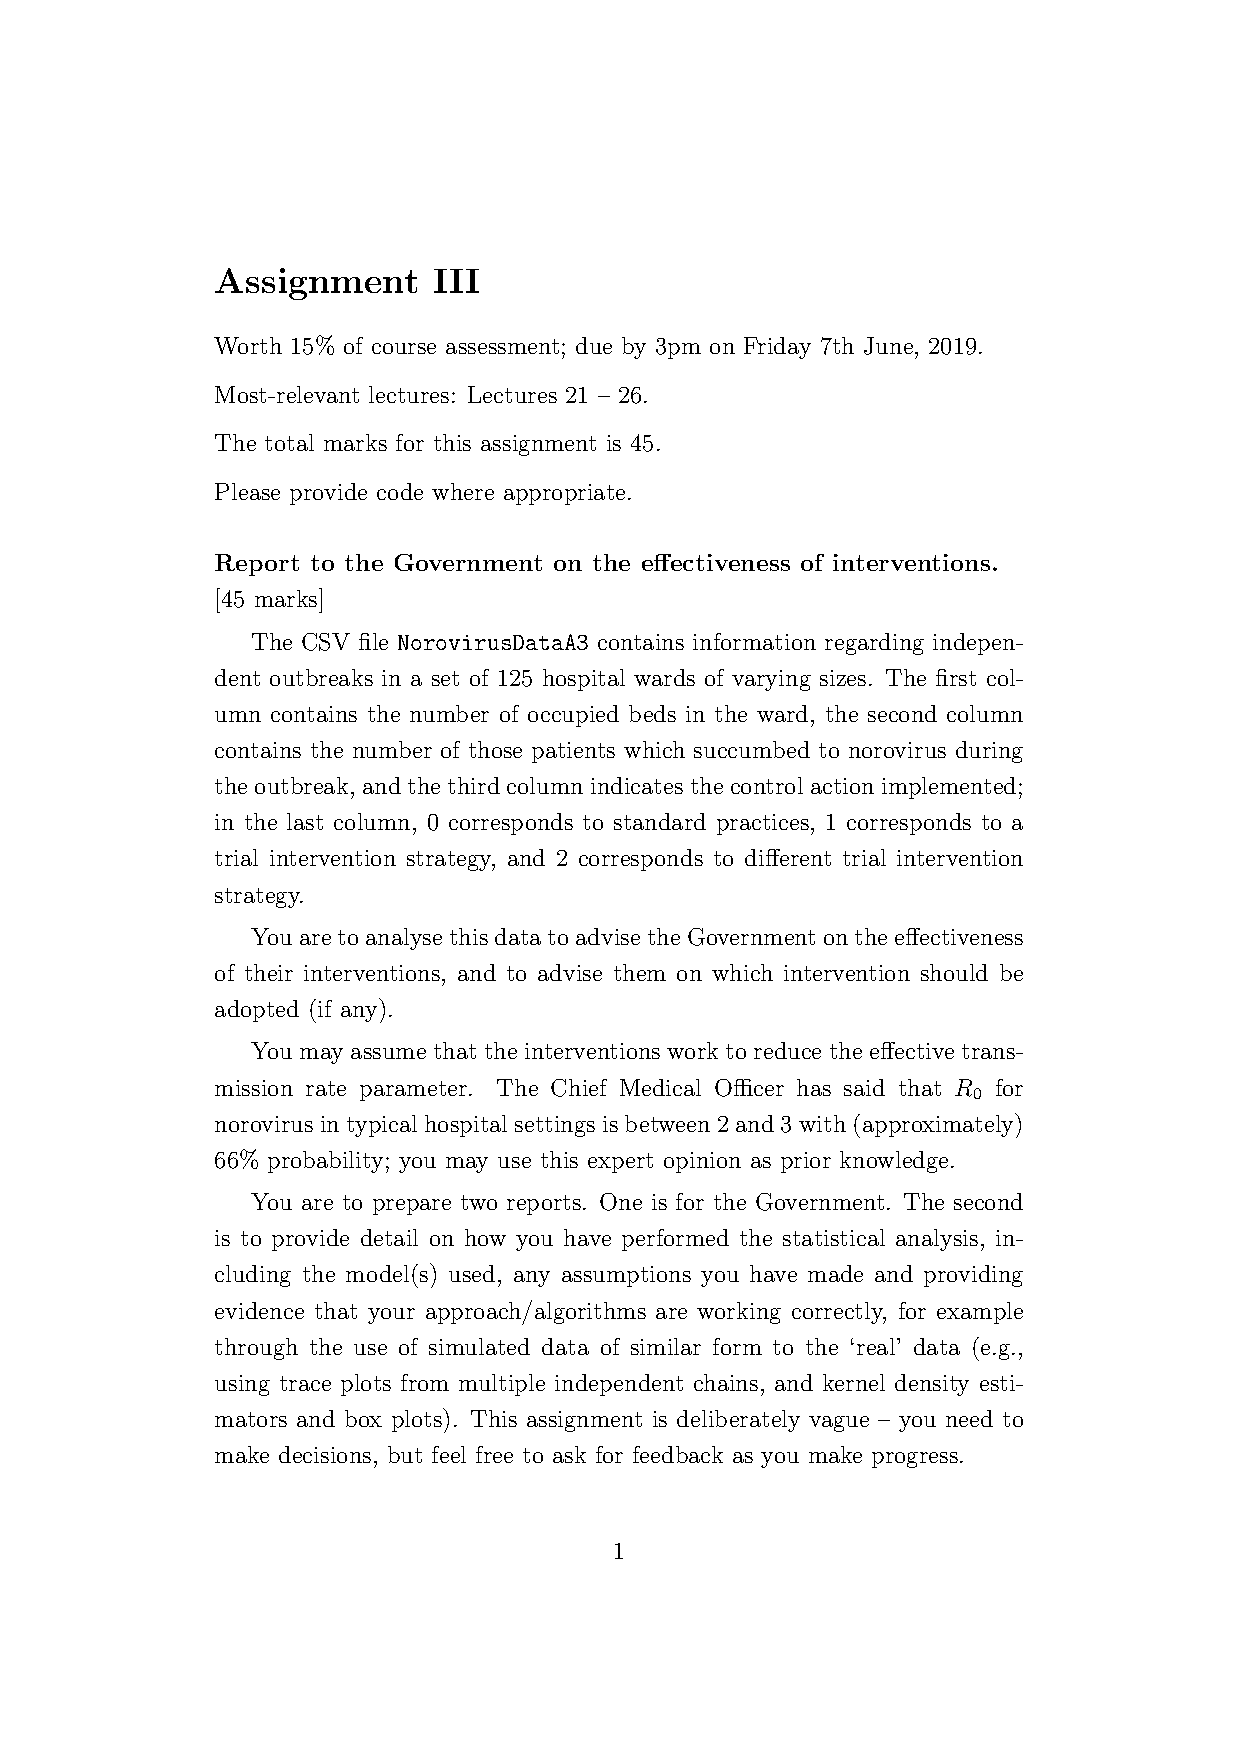
\includepdf[pages=1-]{Honours2019Assignment3}
\end{document}